\chapter{Execute Stage}

\section{Execute}

In the last lab, you created the ALU and ALU Control modules.  Now we will finish the iExecute stage.  The iExecute stage is represented by the red box in Figure ~\ref{fig:execute_stage}.  To finish the iExecute stage, you will need to add the following:
 
\begin{enumerate}
	\item Mux to select the source of the second input into the ALU.  You can reuse your mux that you created in the iFetch stage.
	\item Shifter to left shift the sign extended branch address offset.  You will need to create a new module for this.
	\item Adder to add the branch address offset to the current PC.  You can reuse your adder that you created in the iFetch stage.  Please note the adder is near the top of the datapath diagram and it has an output named ALU result on the diagram.  In fact, this is not a full ALU, but just and adder.  And our output signal will be named branch\_target, as this is what it really is.
\end{enumerate} 

\begin{figure}
	\caption{Execute Stage}\label{fig:execute_stage}
	\begin{center}
		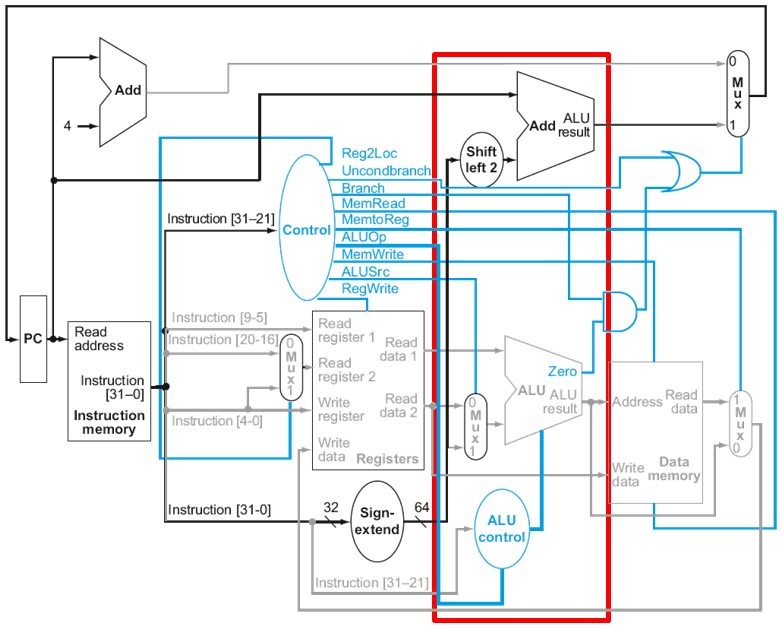
\includegraphics[width=4.75in]{../images/execute_stage.png}
	\end{center}
\end{figure} 

These five modules should be included in a new module called iExecute.  iExecute should consist of everything shown in the red box on Figure ~\ref{fig:execute_stage}. 

The testbench will run the 10 instructions in your Expected Results Table.  Therefore, your next step is to update your Expected Results Table by updating the 3 outputs of the iExecute stage. You also need to update 1 input to the table, PC.  The PC value should start at 0 and increment by 4 for each instruction.  Populate the iExecute output rows with expected values for each instruction.  All of the inputs that you need to determine the expected result are in the table.  Make sure to use N/A if the signal is not applicable for a given instruction.

Finally, you need to complete the testbench.  I have provided the bulk of the testbench.  The only updates that you need to make to the testbench are:
\begin{enumerate}
	\item I have X for all er values right now.  Please update these to the correct values per your Expected Results Table.
	\item I have a verify function call for all 3 outputs for every instruction.  If an output is N/A for a particular instruction, remove or comment out that verify.  There should be a total of 20 test cases.  
\end{enumerate}   


\section{Your Assignment}
You are to:
\begin{enumerate}
\item Complete the iExecute module 
\item Update your Expected Results Table with the outputs from the iExecute stage.  Also add a PC value. 
\item Update iExecute\_test.sv
\item Verify that your simulation results match your expected results.
\item Rather than writing a lab report, please produce a landscape mode PDF file called Lab9\_lastname.pdf that includes (in this order):
\begin{enumerate}
	\item Your name and the lab number.
	\item A snip of your completed Expected Results Table.
	\item A snip of the Simulation Results for the iExecute test.  Please show instructions in hex, opcodes and control signals in binary and everything else in signed decimal.  
	\item Copy and paste the entire log from BEGIN TEST RESULTS to END TEST RESULTS into your file.  The results have gotten too long to use the snipping tool.	
\end{enumerate}
\item Upload Lab9\_lastname.pdf file to Canvas.
\item Zip up your ARM-Lab directory and submit it on Canvas as well.  I will run your code against my correct testbench to verify that your code and testbench work correctly.

\end{enumerate} 